\documentclass{standalone}
\usepackage{tikz}
\usepackage{ctex,siunitx}
\setCJKmainfont{Noto Serif CJK SC}
\usepackage{tkz-euclide}
\usepackage{amsmath}
\usetikzlibrary{patterns, calc}
\usetikzlibrary {decorations.pathmorphing, decorations.pathreplacing, decorations.shapes,}
\begin{document}
\small
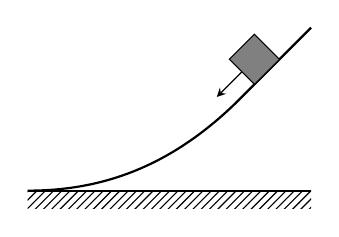
\begin{tikzpicture}[>=stealth,scale=0.9]
  \useasboundingbox(0,-0.25)rectangle(4,2.3);
  \fill [pattern = north east lines] (0,-0.25) rectangle (4,0);
  \draw[thick](0,0)--(4,0); 
  \draw[thick](4.0,2.3)--(3.0,1.3)..controls(2.0,0.3)and(1.0,0.0)..(0,0); 
  \draw [fill=gray] (3.2,1.5)--++(45:0.5)--++(135:0.5)--++(225:0.5)--cycle;
  \draw [->] ([shift=(135:0.25cm)]3.2,1.5)--++(225:0.5);
\end{tikzpicture}
\end{document}